\chapter{EG4 run}
\label{cha:EG4}

The deuteron target part of the EG4 experiment ran for about a month in 2006, mostly with %the 
longitudinally polarized frozen $^{15}$ND$_3$ as the target% with the CLAS torus field in the electron outbending setting (-1500A and -2250A respectively for 1.3 and 2.0 GeV cases)  in order to achieve very low \qsqs measurements by detecting electrons at as low forward scattering angles as possible (down to $\theta=6$ degrees)
. In between these deuteron runs, some small amount of data was %were (amount is a singular, not data, at least to SEK)
also collected on carbon-12 and empty cell targets, which are important in various auxiliary studies during the data analysis (such as their use in estimating nuclear background while developing momentum corrections, estimating the length %size 
of the target material %(Banjo length study),
 or estimating unpolarized background). %in other analysis works). 
 A total of 113 data runs (from run ID 51896 to 52040) were collected for the lower beam energy (1.3 GeV) and 221 runs (from 51593 to 51867) for the 2.0 GeV case (with each run consisting of %collecting data from %GED
 about $3.0\times 10^7$ event triggers) \cite{eg4wiki}. %113 runs for 1.3 GeV and 221 (each run 
Each run took about 2 hours and collected about 2 GB of data in %the 
raw format and saved as about 20-30 BOS files (see next section). With the combination of low %values of 
beam energies and low scattering angles, % measurement, 
low momentum transfers can be measured down to about 0.02 GeV$^2$ %are achieved 
within the kinematic coverage of the resonance region ($1.08 ~ < W <2.0$ GeV.) % \lessapprox 2.0$). 



In addition to the use of low beam energies and low $\theta$ measurements, in order to maximize the statistics in the low momentum transfers, following measures were taken that were unique to the experiment:
\begin{itemize}
\item Use of the electron outbending torus field configuration to enhance the low angle acceptance (so that more of very forward going electrons would be bent towards and detected by the CLAS detector).
\item Use of a a newly built Cerenkov Counter (CC) in the $6^{th}$ sector\footnote{For reasons of limited resources, only one new CC was built and the $6^{th}$ sector alone was used to detect the scattered electrons} (see Figs. \ref{nwCcCAD} and \ref{figcherenkovNw}) that was designed to optimize electron detection in the outbending torus configuration. %such that the %sek
This led to a better and more uniform %sek
  detection efficiency would be better and more uniform than with the existing counters\footnote{The standard CLAS Cherenkov detectors were designed such that their optics, geometry, module position and mirror orientation were optimized for low rate high \qsq experiments that mostly use(d) electron in-bending torus fields. The design was a compromise between the desired kinematic coverage and the complexities of the CLAS detector system including the effect of the torus field.} which were optimized for electron inbending configuration. 
\item To further enhance the low angle coverage, the polarized target was placed in a more retracted position along the beam line i.e. at about -101.0 cm upstream of the CLAS center.
\end{itemize}

Other than that the CLAS detector was used in the standard configuration like in any other polarized target experiments using CLAS. The following list summarizes various specifications of the experimental setup (for more details see \cite{anaNoteXZheng}):
\begin{itemize}
\item \textbf{Beam energies:} 1.3 and 2.0 GeVs for ND$_3$ target runs and 1.0, 1.3, 2.0, 2.3 and 3.0 GeVs for NH$_3$ target runs.
\begin{itemize}
\item \textbf{Beam polarization: } Longitudinally polarized ($\approx 85\%$) electron beam from CEBAF accelerator. Moeller scattering used for the polarization measurement.
\end{itemize}
\item \textbf{Polarized targets: } Solid ND$_3$, and NH$_3$ targets polarized using the technique of Dynamic Nuclear Polarization (DNP).
\begin{itemize}
\item \textbf{Average polarizations: } Between (75 - 90)$\%$ and  (30 - 45)$\%$ respectively.
\item \textbf{Lengths: } 1cm for ND$_3$ and 1 cm and 0.5 cm for  NH$_3$.
\item \textbf{Densities: } 1.056 and 0.917 respectively.
%Packing fraction from Sarah's wiki page: https://clasweb.jlab.org/rungroups/eg4/wiki/index.php/October_28,_2011
\item \textbf{Packing fractions: } (0.624, 0.764) for (1.3, 2.0) GeV  ND$_3$ runs respectively and (0.625, 0.624/0.717\footnote{The two numbers 0.624/0.717 for the 1.3 GeV NH$_3$ runs are due to the fact that two different NH$_3$ targets were used in case of 1.3 GeV runs. One target was in the top cell and the other was in the bottom cell of the target stick.}, 0.716, 0.682, 0782) for (1.0, 1.3/1.3, 2.0, 2.3, 3.0) GeV NH$_3$ runs.  
\end{itemize}  
\item \textbf{Other targets: } Carbon-12 (1 cm and 0.5 cm long), Empty target cup, Target cup filled only with liquid helium (LHe), LHe bath and various foils due to different target chamber windows. 
\item \textbf{Torus currents: } 1500 Amps for 1.0 and 1.3 GeV runs and 2250 A for 2.0, 2.3, and 3.0 GeV runs.
\end{itemize}  
%\subsection{Cherenkov Counters (CC)}

\begin{comment}

\begin{figure}[hp]
\centering
\subfigure[Standard CC module]{% other than $6^{th}$ sector]{
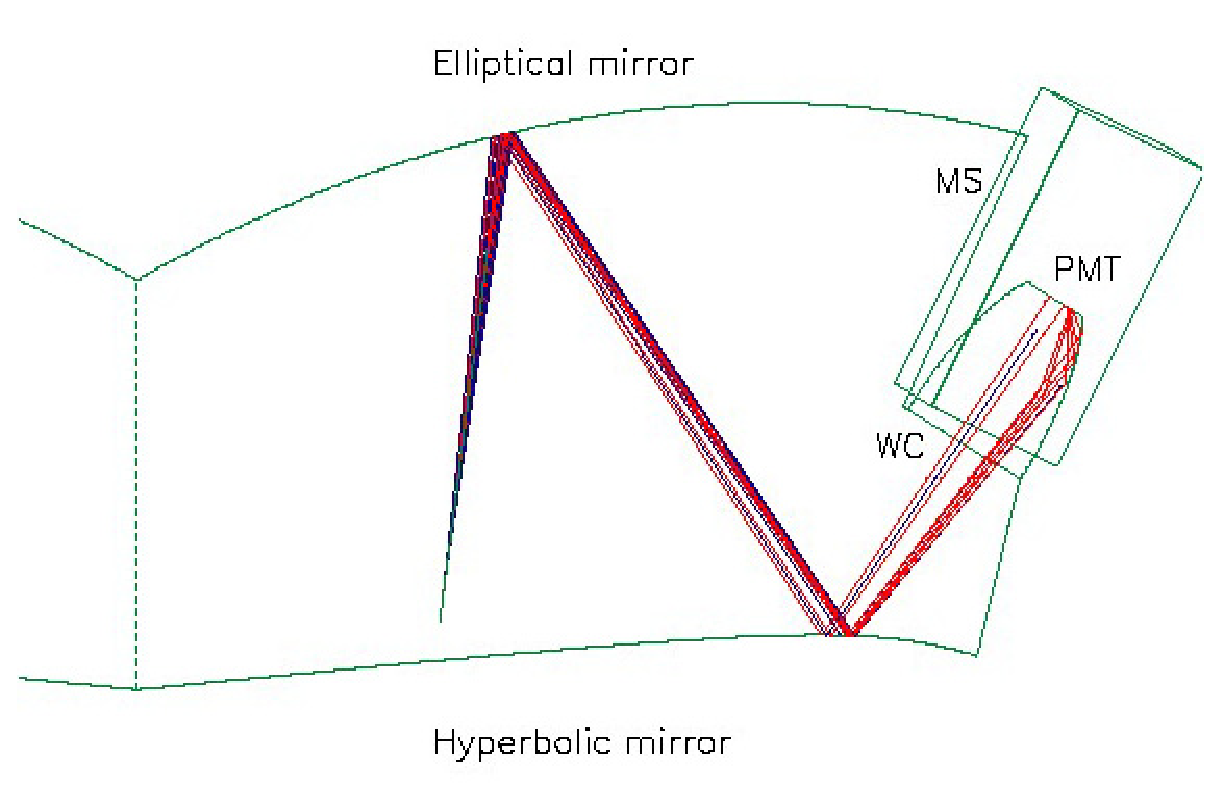
\includegraphics[scale=0.25]{chap6expSetup/Figures/ccmodule.eps}
\label{figccmodule}
}
\subfigure[A CC segment of the standard CC]{
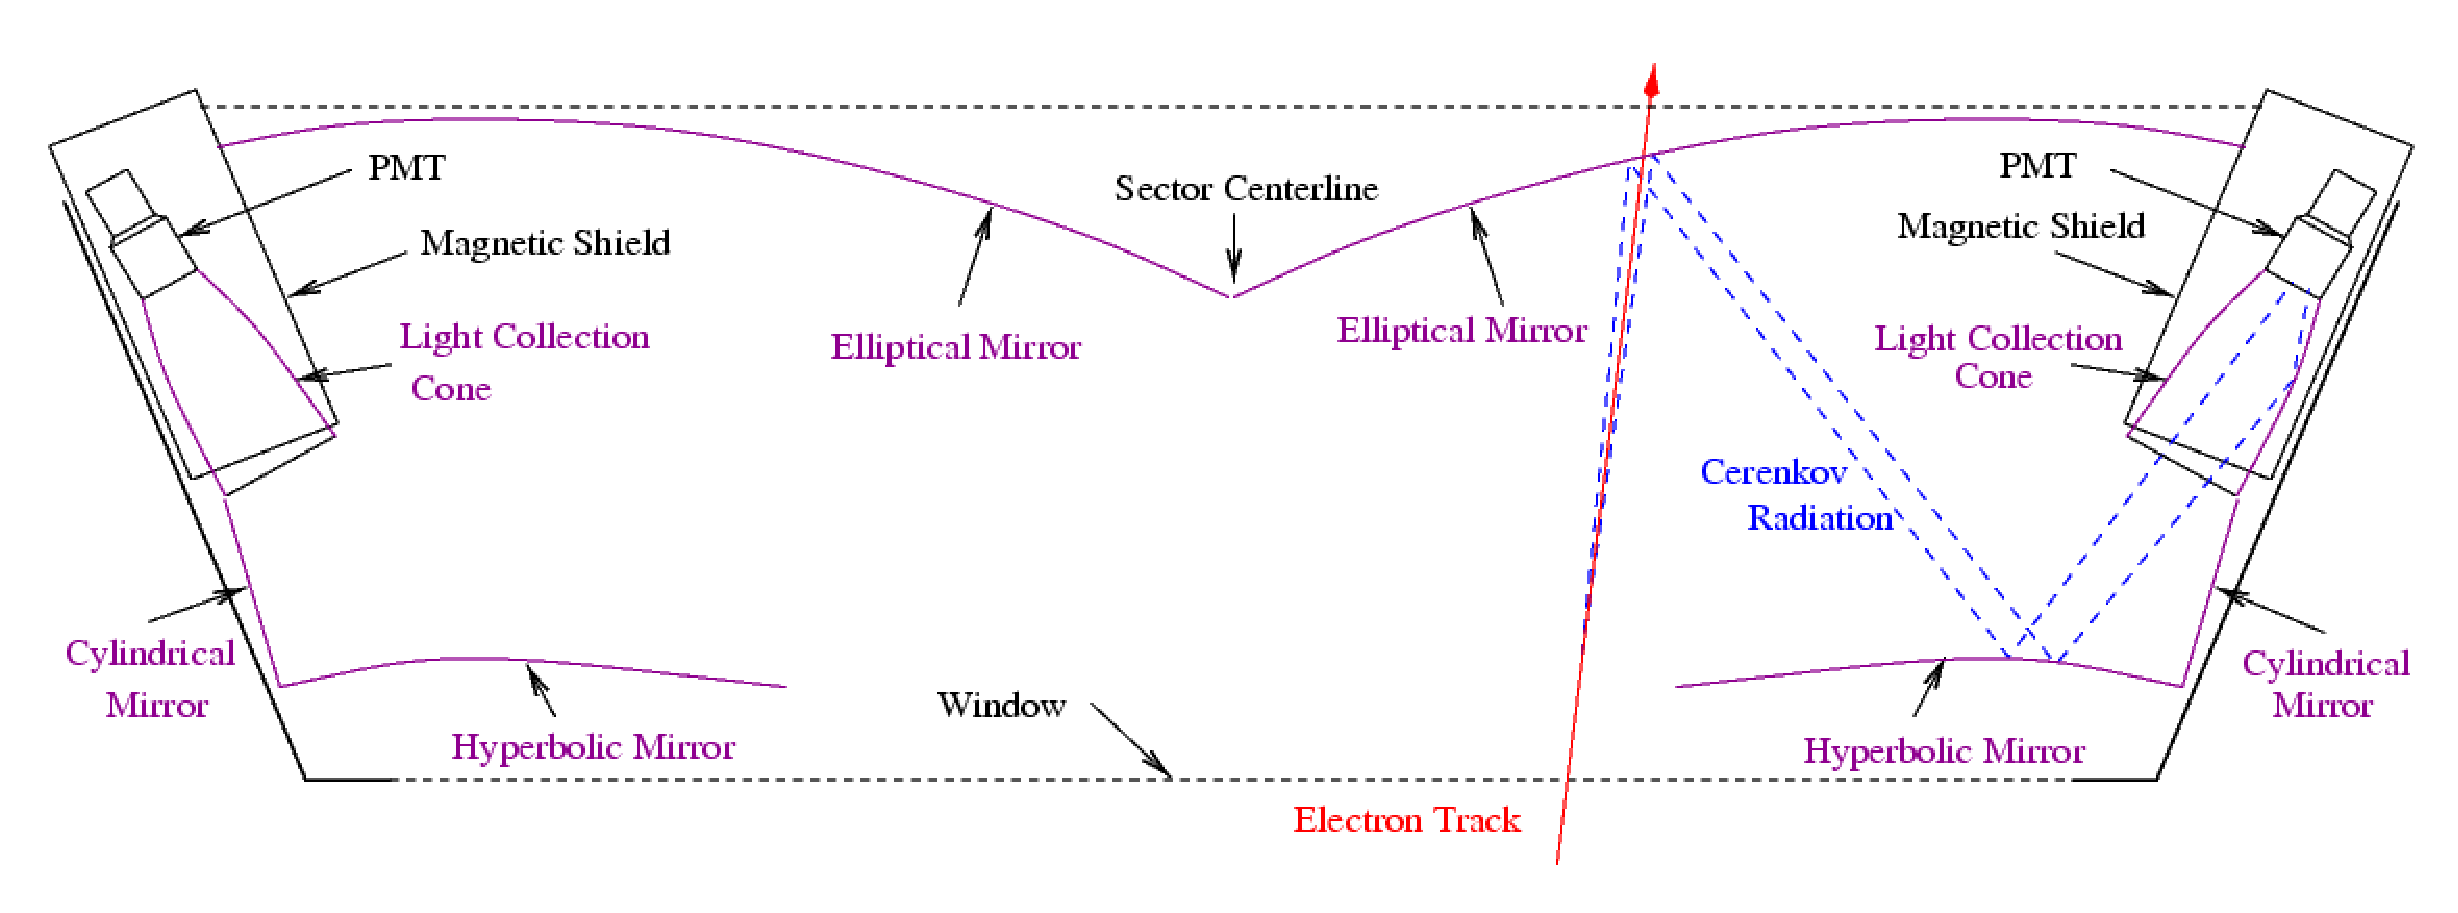
\includegraphics[scale=0.22]{chap6expSetup/Figures/ccsegment.eps}
\label{figccsegment}
}
\label{figcherenkov} %Effect of Dc-smear
\caption[A Cherenkov Counter module]{A Cherenkov Counter (CC) module in CLAS.}
\end{figure}

\end{comment}




\begin{figure}[h] %ht, htpb (p - float, b = bottom, h=? t = top)
\centering
%\leavevmode 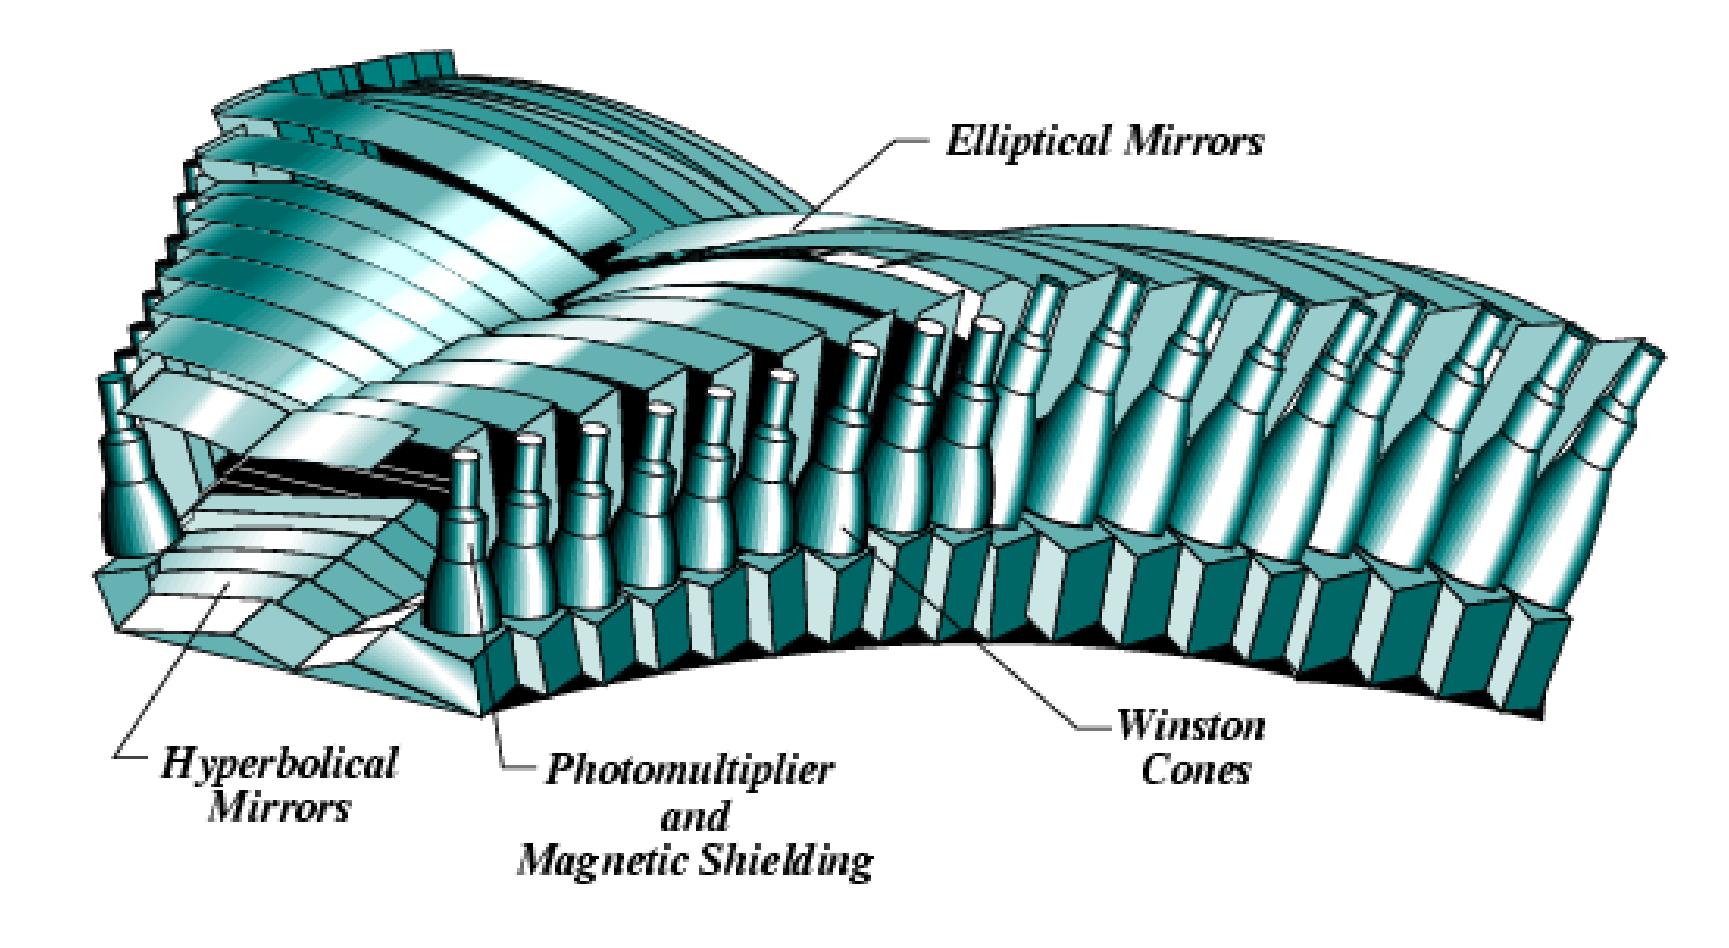
\includegraphics[width=0.8\textwidth]{chap6expSetup/Figures/ccunit.eps}  %0.6 is the fraction of the real image width????
\leavevmode 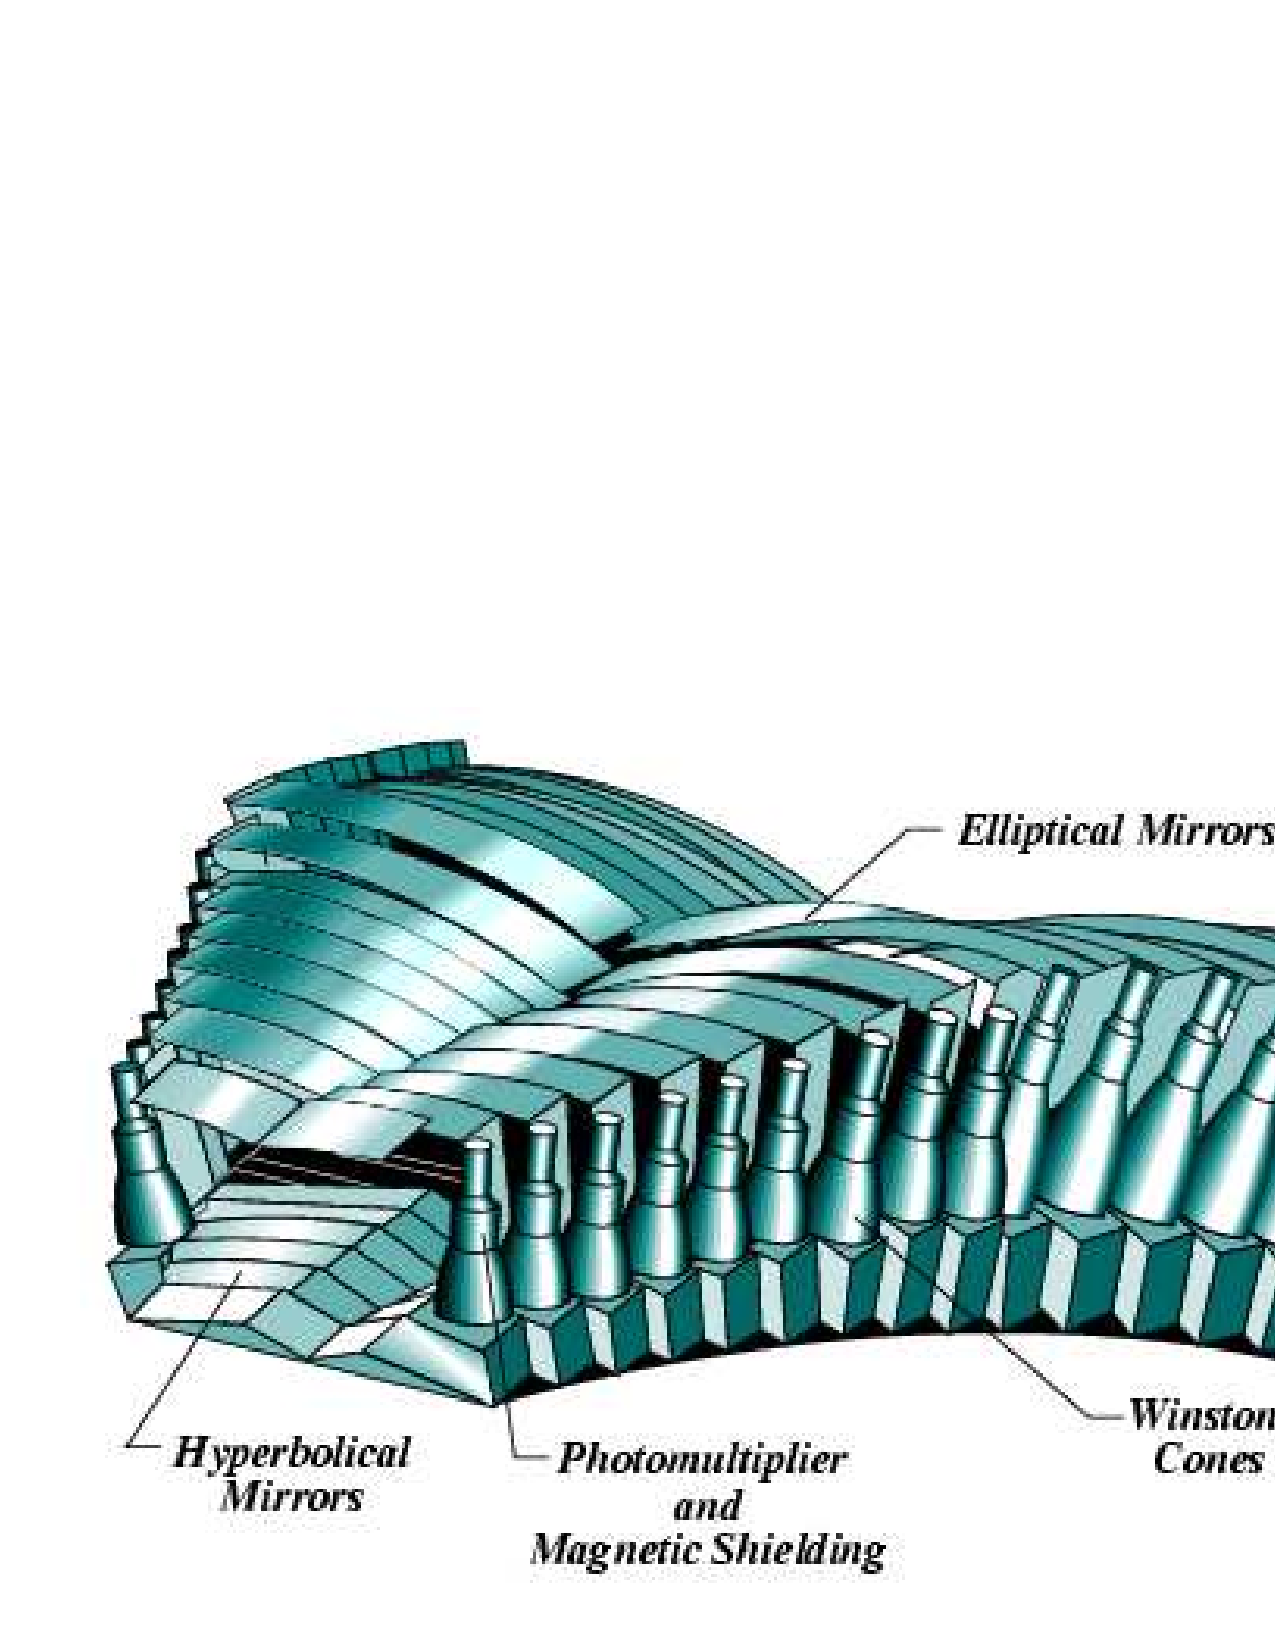
\includegraphics[width=0.8\textwidth]{figuresEG4/FigExp/ccunit.pdf}  %0.6 is the fraction of the real image width????
\caption[The Standard CLAS Cherenkov Counter]{The computer rendered image of the Standard CLAS Cherenkov Counter}
\label{figcherenkov}%{figccunit}
\end{figure}

\begin{comment}
%\pagebreak   %12/6/13 (because nothing else that I tried worked)

%Threshold Counter https://en.wikipedia.org/wiki/Cherenkov_radiation#Particle_physics_experiments 
The Cherenkov Counters (CC) serve the dual function of triggering on electrons and separating electrons from pions (or identifying charged particles). These detectors use the light emitted by Cherenkov radiation (emission of light when the charged particle travels faster than light in that medium) to measure the particle velocity (and, therefore, $\beta=v/c$). The knowledge of $\beta$ combined with the particle momentum (from the tracking detectors) determines the particle's mass, thus giving us information on %the clue for %SEK
the particle identification. %ID. %GED
%Choosing different gases to fill in, the %GED
The index of refraction (n) is carefully optimized for the particle masses and momentum range of the experiments in question. Threshold counters record all light produced, thus providing a signal whenever $\beta$ is above the threshold $\beta_t$ = 1/n. In the standard configuration, CLAS uses one Cherenkov threshold detector in each of the six sectors in the forward region from $8^o$ to $45^o$.


\end{comment}
\begin{figure}[h] %ht, htpb (p - float, b = bottom, h=? t = top)
\centering
\leavevmode 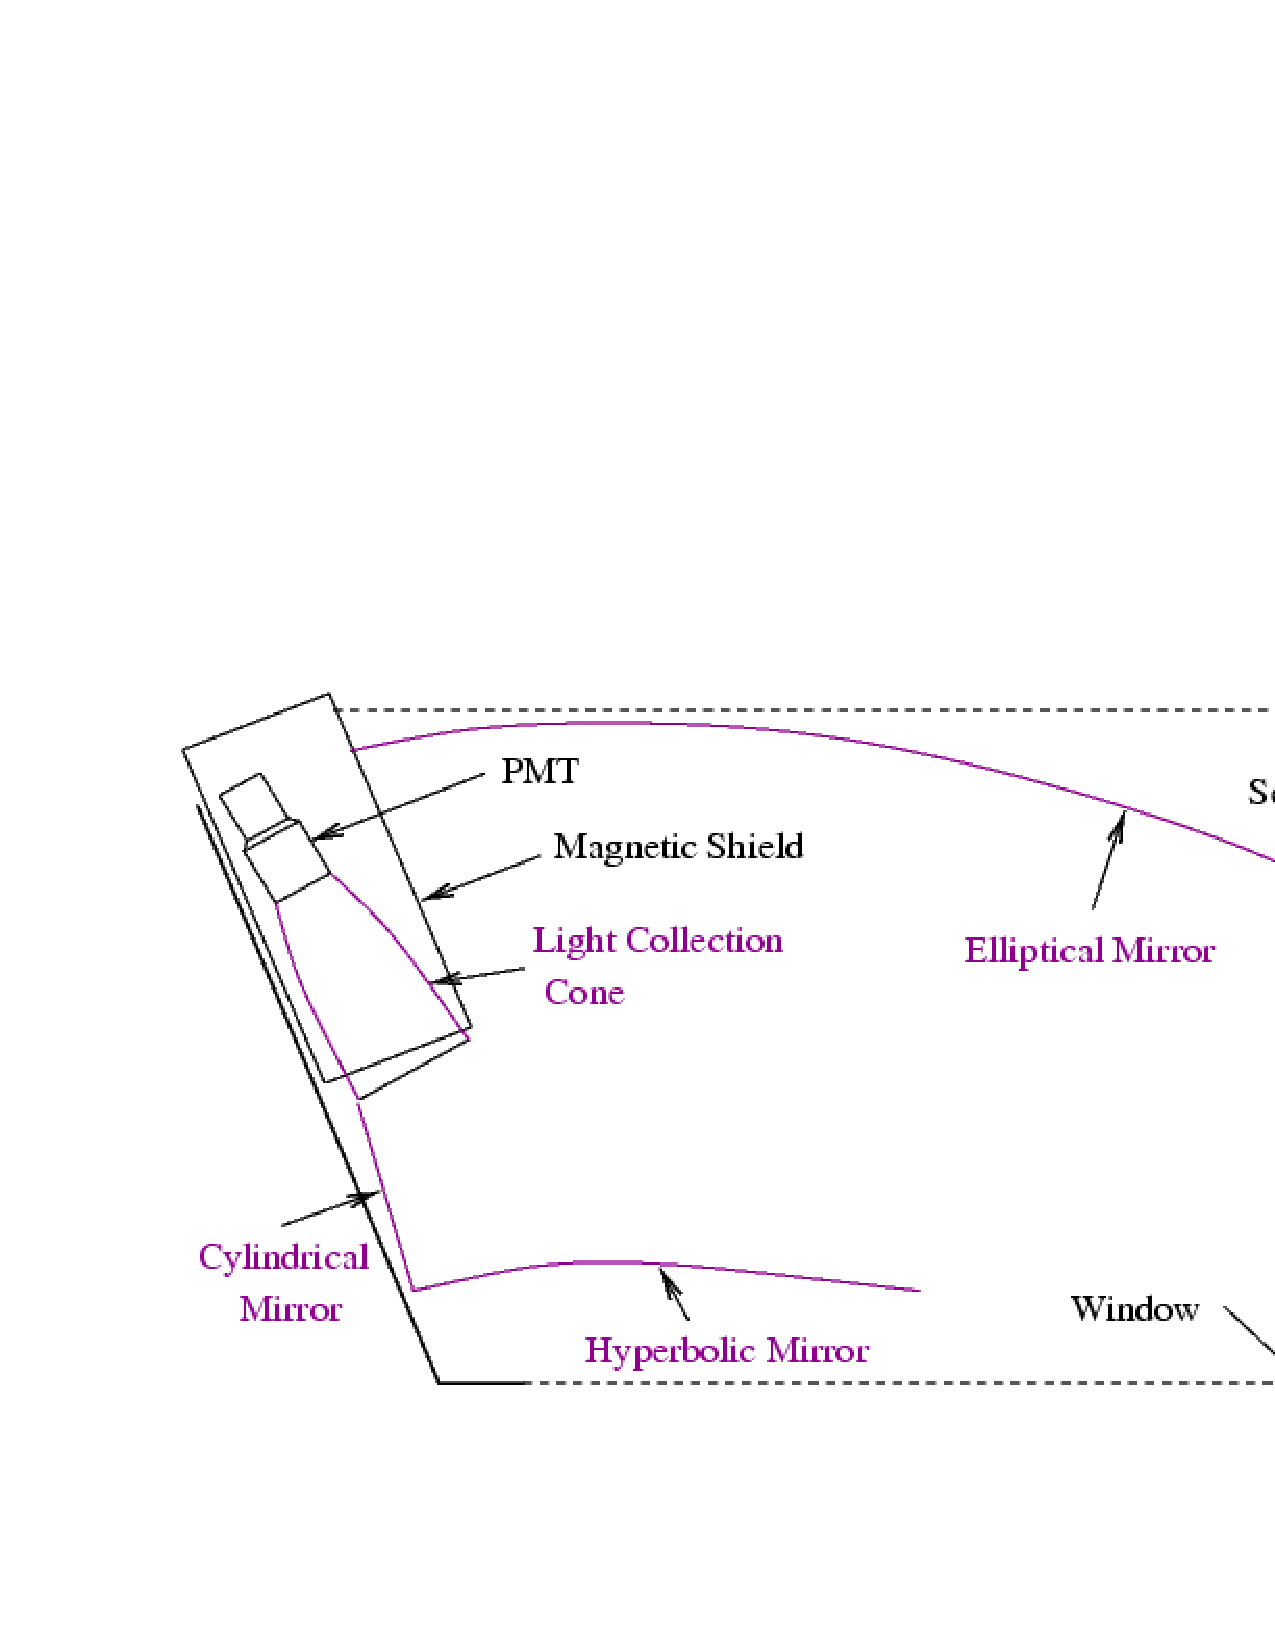
\includegraphics[width=1.0\textwidth]{figuresEG4/FigExp/ccsegment}  %0.6 is the fraction of the real image width????
\caption[A Cherenkov Counter module]{The schematic diagram of a CLAS Cherenkov Counter (CC) module showing mirrors, PMTs and the light reflections. %\textcolor{red}{Changed}
}
\label{figccunit}%{figcherenkov}
\end{figure}







%\subsubsection{New CC in the $6^{th}$ Sector}
\section{New CC in the $6^{th}$ Sector}
\label{newCCsec}
%Threshold Counter https://en.wikipedia.org/wiki/Cherenkov_radiation#Particle_physics_experiments 
The Cherenkov Counters (CC) serve the dual function of triggering on electrons and separating electrons from pions (or identifying charged particles). These detectors use the light emitted by Cherenkov radiation (emission of light when the charged particle travels faster than light in that medium) to measure the particle velocity (or rather $\beta=v/c$). The knowledge of $\beta$ combined with the particle momentum (from the tracking detectors) determines the particle's mass, thus giving us information on %the clue for %SEK
the particle identification. %ID. %GED
%Choosing different gases to fill in, the %GED
The index of refraction (n) is carefully optimized for the particle masses and momentum range of the experiments in question. Threshold counters record all light produced, thus providing a signal whenever $\beta$ is above the threshold $\beta_t$ = 1/n. In the standard configuration, CLAS uses one Cherenkov threshold detector in each of the six sectors in the forward region from $8^o$ to $45^o$.



\begin{comment} %Partly redundant with \footnote and also too verbose as per SEK
The standard CLAS Cherenkov detectors (as shown by Figs. \ref{figcherenkov} and \ref{figccunit}) were designed such that their optics, geometry, module position and mirror orientation were optimized for low rate high \qsq experiments that mostly use(d) electron in-bending torus fields. The design was a compromise between the desired kinematic coverage and the complexities of the CLAS detector system including the effect of the torus field. As a consequence, light collection is constrained causing the number of photoelectrons to be strongly dependent on scattering angles, and making the detection efficiency non-uniform, and strongly reduced in some regions (for example, up to 30\% drop in the middle of the sector and at forward angles) \cite{propE03_006}. While it would still be possible to detect electrons, the use of the existing CC would mean that the absolute cross-section measurement would require large and complex corrections which are difficult to evaluate. %be evaluated. In addition, that %SEK
That would significantly contribute to the systematic uncertainties, thus not meeting the proposed high accuracy requirement of the measurements.
\end{comment}

\begin{figure}[h] %ht, htpb (p - float, b = bottom, h=? t = top)
\centering
%Cut out of the designers CAD rendering of the new CC detector http://www.jlab.org/Hall-B/secure/eg4/ripani/Reference/assieme_totale.jpg
%\leavevmode 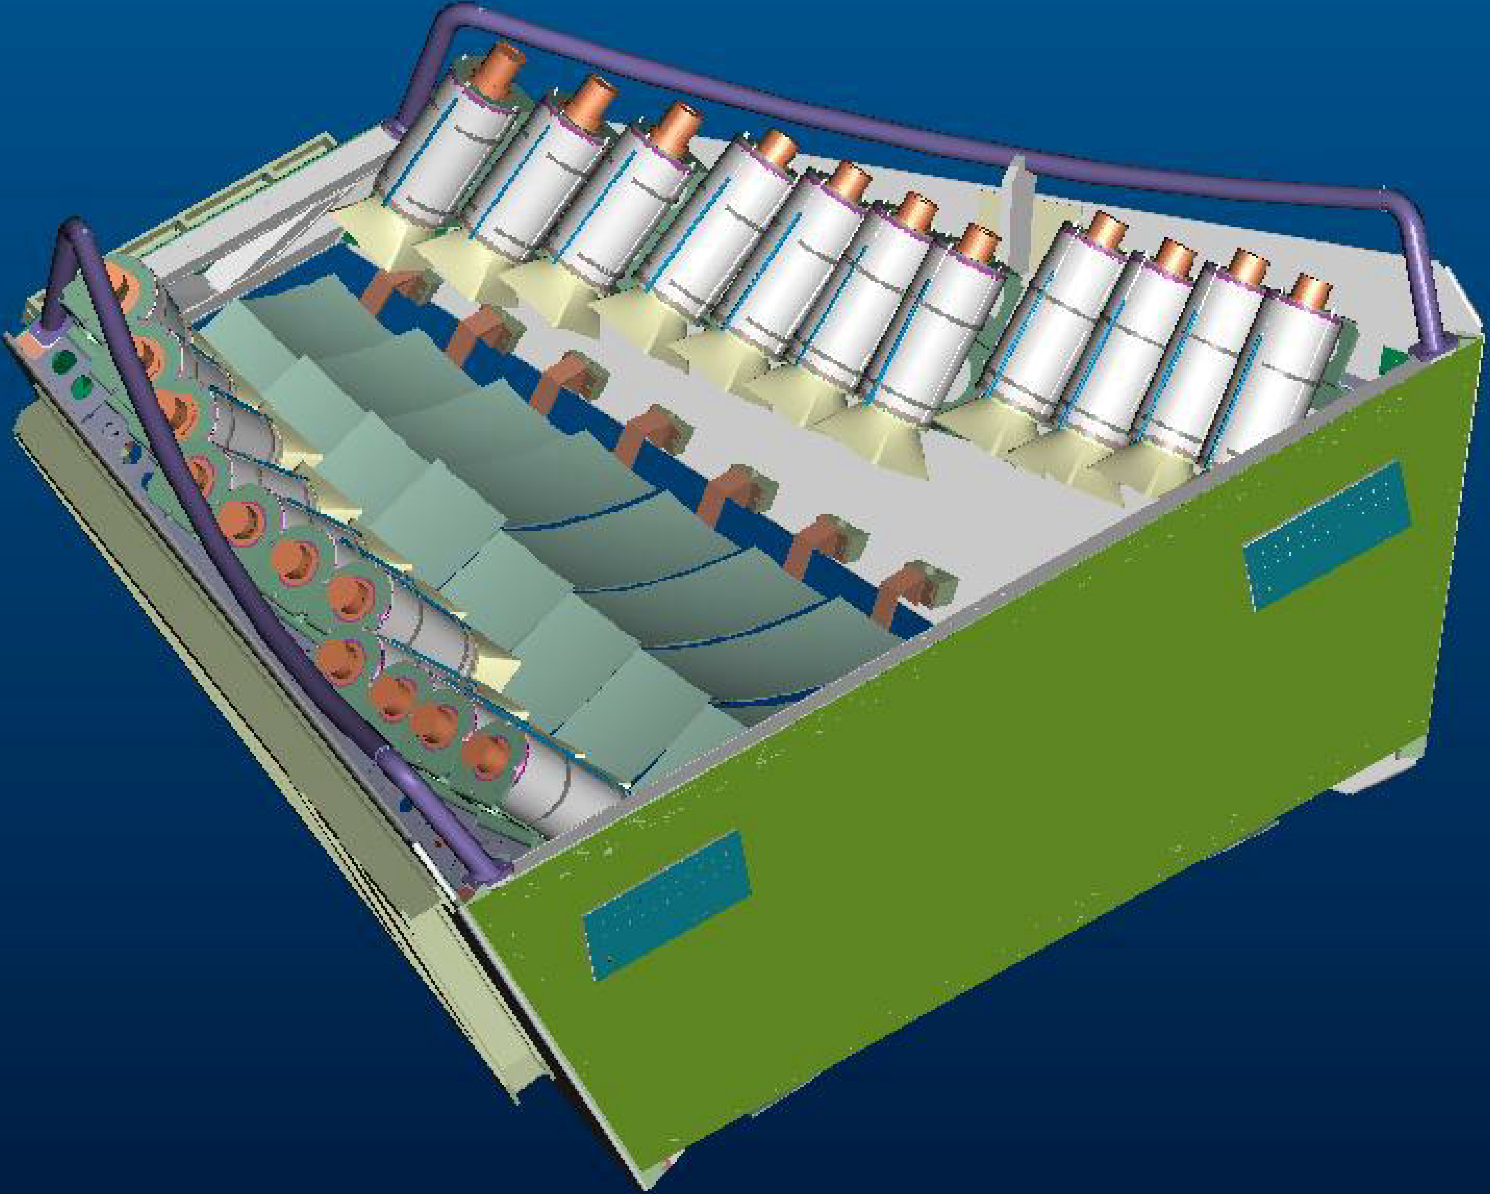
\includegraphics[width=0.8\textwidth]{figuresEG4/FigExp/assieme_totaleCut.pdf}  %0.6 is the fraction of the real image width????
\leavevmode 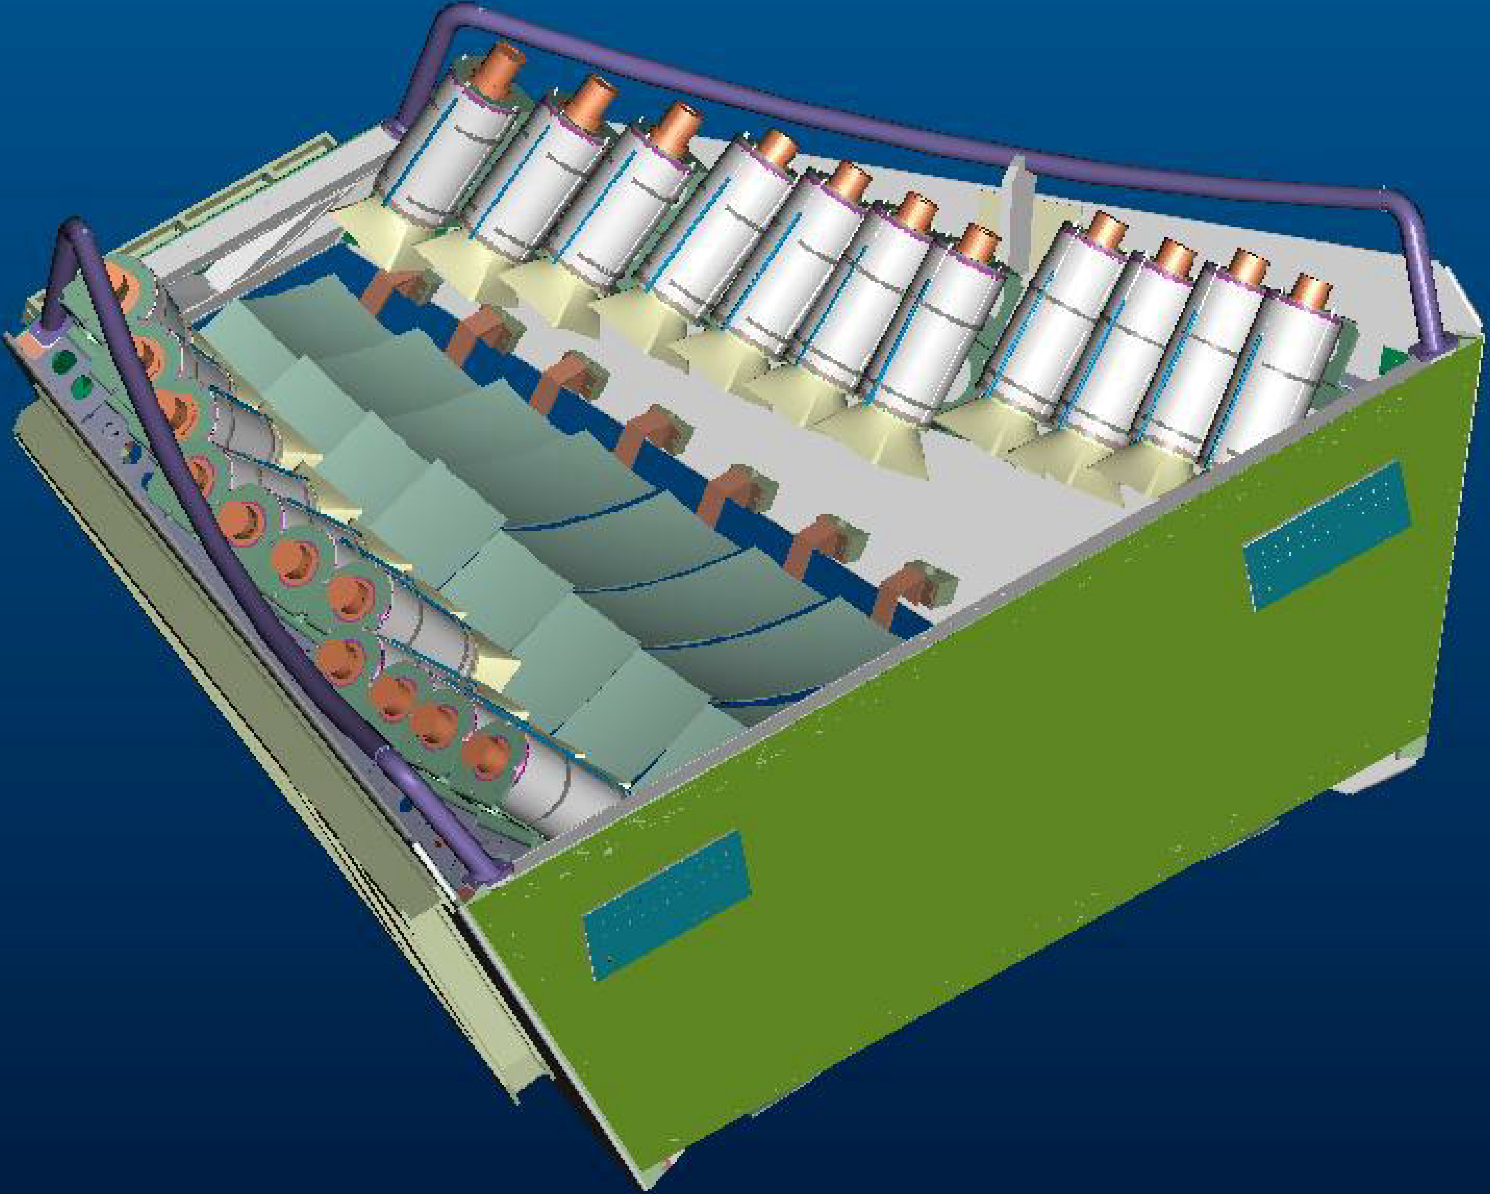
\includegraphics[width=0.8\textwidth]{figuresEG4/FigExp/assieme_totaleCut.pdf}  %0.6 is the fraction of the real image width????
%\leavevmode 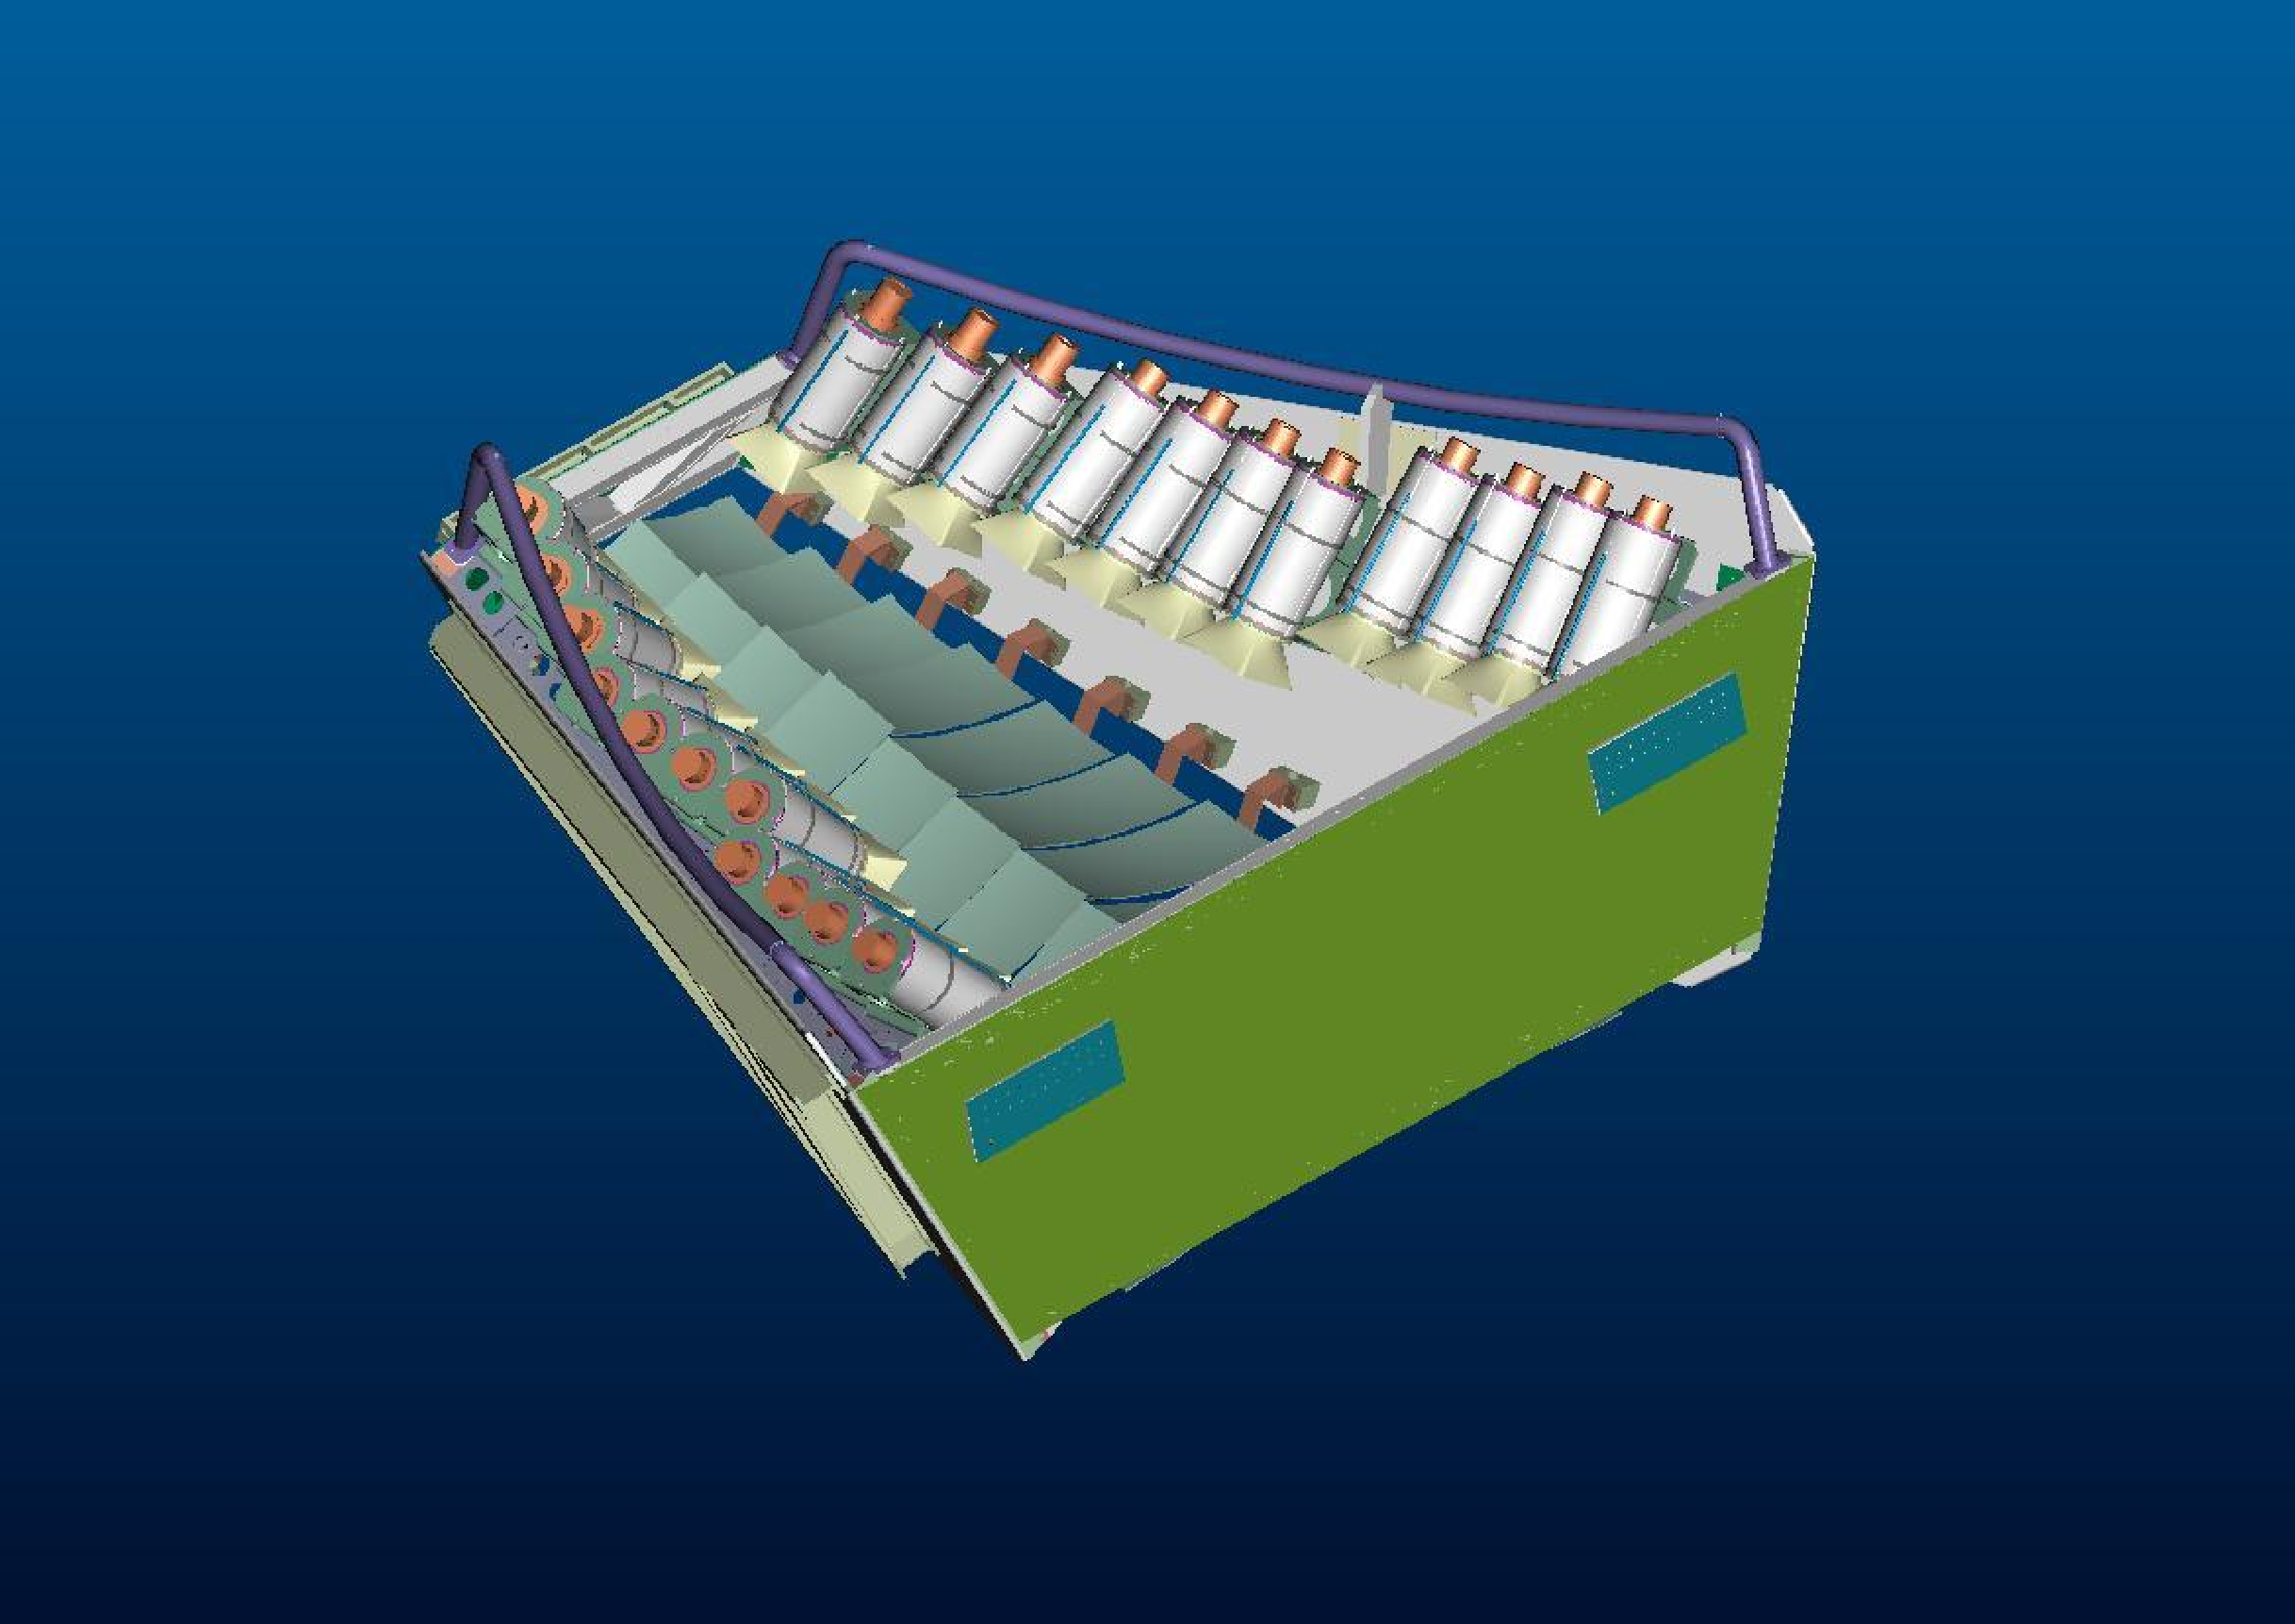
\includegraphics[width=0.8\textwidth]{figuresEG4/FigExp/assieme_totale.pdf}  %0.6 is the fraction of the real image width????
%\includegraphics[trim={5cm 0 0 0},clip]{example-image-a}  %http://tex.stackexchange.com/questions/57418/crop-an-inserted-image
\caption[New Cherenkov counter]{The new Cherenkov counter (courtesy of INFN, Genova)}
\label{nwCcCAD}
\end{figure}



%In order to avoid having all those CC-related issues in the new measurements, a
A new gas threshold cherenkov counter (designed and built by INFN - Genova, Italy) was installed in the sixth sector. %, with no further modifications of the CLAS. 
This new CC detector (see Fig. \ref{nwCcCAD} for its CAD rendition) is specifically optimized for the out-bending field configuration, which is necessary to reach the desired low momentum transfer (measurements down to 6 degrees). The detector uses the same radiator gas ($C_4 F_{10}$ - perfluorobutane) and the same gas flow control system as the standard %old
one, but it uses a %completely %SEK
different design. %, including mirror types and orientation for light reflection and 
In the new CC, the number of CC-modules %/units 
is now 11 instead of the 18 in the standard ones. In order to maximize the light collection, a single reflection design (see Fig. \ref{newCCphRefl}) using spherical mirrors is used (the standard CC used double relections from elliptical and hyperbolic mirrors). The geometry, the size, the mirror size, position, and orientation, the dimensions as well as the assembly of the modules were optimized for the experiment %using a dedicated FORTRAN code 
and the performance study was %also 
done using a complete GEANT simulation \cite{propE03_006}. Additionally, for the purpose of efficiency and performance studies (see Sec. \ref{secCCineff}), a few special trigger data runs were taken during the experiment. These special runs had the trigger that mainly involved EC-signals (and no CC-signal at all) to decide whether the detected particle was a good scattered electron candidate.


\begin{figure}[h]
\centering
\subfigure[Schematic of a new CC segment.]{
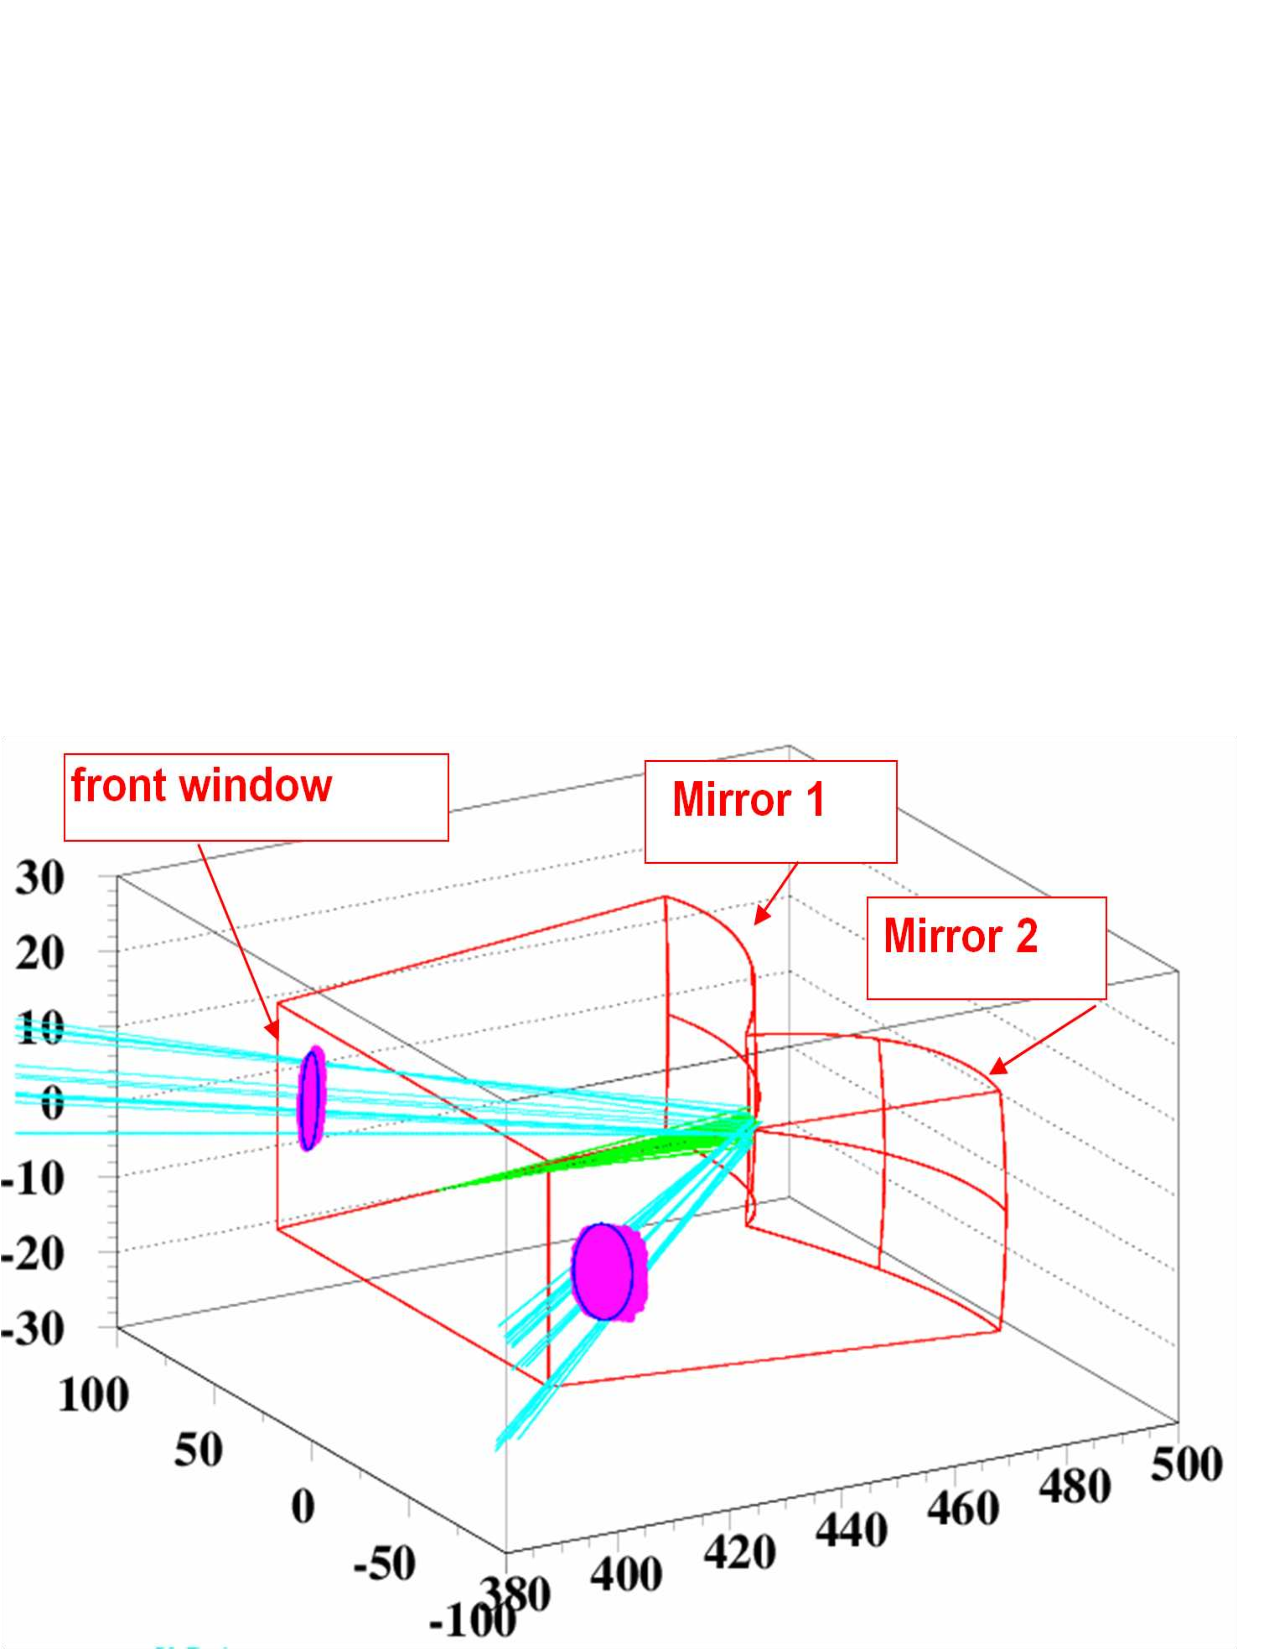
\includegraphics[scale=0.32]{figuresEG4/FigExp/newCCmoduleLights}
\label{nwCCunit}
}
\subfigure[Schematic of light reflections.]{
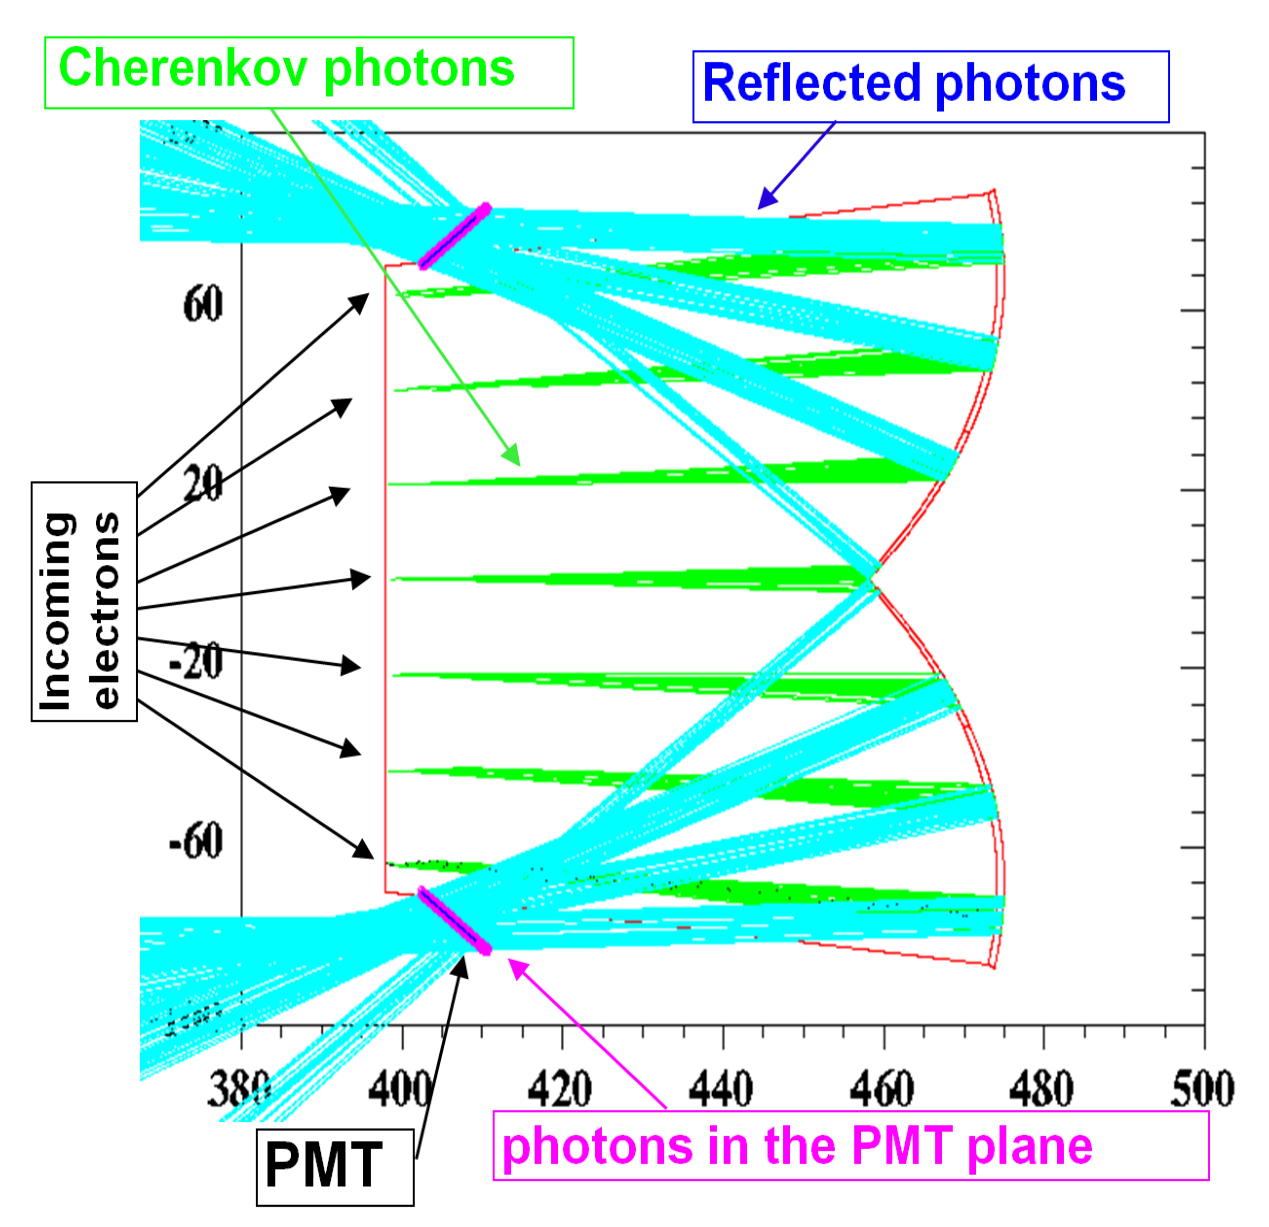
\includegraphics[scale=0.28]{figuresEG4/FigExp/cerenkovLightReflection}
\label{newCCphRefl}
}
\caption[A new CC segment and light reflections]{Schematic of a new CC segment showing the arrangements of the mirrors, PMTs and the light reflections (courtesy of INFN, Genova).}
\label{figcherenkovNw} %Effect of Dc-smear
\end{figure}


%This new detector achieves a very high and uniform electron detection efficiency ($\approx$ 99.9\%) in most of its central (fiducial) region, to allow for the measurement of the absolute cross-section with minimal corrections and a high pion rejection ratio (of the order of $10^{-3}$). Due to the high electron rate at low \qsq, the \ph coverage can be lowered, while still having a large counting rate. %, we will have an overwhelmingly large amount of scattering at smaller angles, 
%Therefore, for reasons of limited data storage capability, and also for the fact that only the sixth sector had the required new CC, only the sixth sector events were collected, stored and subsequently used for data analysis.% \cite{jlabVocab_wb}.

